\documentclass[10pt]{beamer}

\usepackage[english]{babel}
\usepackage[utf8]{inputenc}
\usepackage[T1]{fontenc}
\usepackage{lmodern}

\usepackage{layout}
\usepackage{epsfig}
\usepackage{graphicx}
\graphicspath{{images/}}

\usepackage{siunitx}

\usepackage{amsthm}
\usepackage{amsmath}
\usepackage{amssymb}

\usepackage{mathrsfs}
\usepackage{wrapfig}
\usepackage{url}
\usepackage{multirow}
\usepackage{array}
\usepackage{pgfplots}

\usepackage[version=3]{mhchem}

\usepackage{wasysym}

%Bibtex
%\usepackage[square]{natbib}
%\newcommand{\newblock}{}

\usetheme{Warsaw}

\usepackage{graphicx}
\usepackage{epsfig}
\usepackage{epstopdf}
%\DeclareGraphicsRule{.eps}{pdf}{.pdf}{`epstopdf #1}
%\pdfcompresslevel=9
%\epstopdfsetup{suffix=}

\usepackage[]{algorithm2e}

\usepackage{todonotes}
\title{PageRank}
\author{
  Quentin Laurent
  \and
  Benoît Legat
}

\newcommand\bigoh{\mathcal{O}}

\usepackage{tikz}
\tikzstyle{vertex}=[circle,fill=gray!50,minimum size=15pt,inner sep=0pt]
\tikzstyle{visited}=[circle,fill=green!25,minimum size=15pt,inner sep=0pt]
\tikzstyle{unvisited}=[circle,fill=blue!25,minimum size=15pt,inner sep=0pt]



\begin{document}

\begin{frame}
  \maketitle
\end{frame}
\begin{frame}
  \tableofcontents
\end{frame}
\section{Introduction to pagerank}
\setbeamertemplate{background canvas}{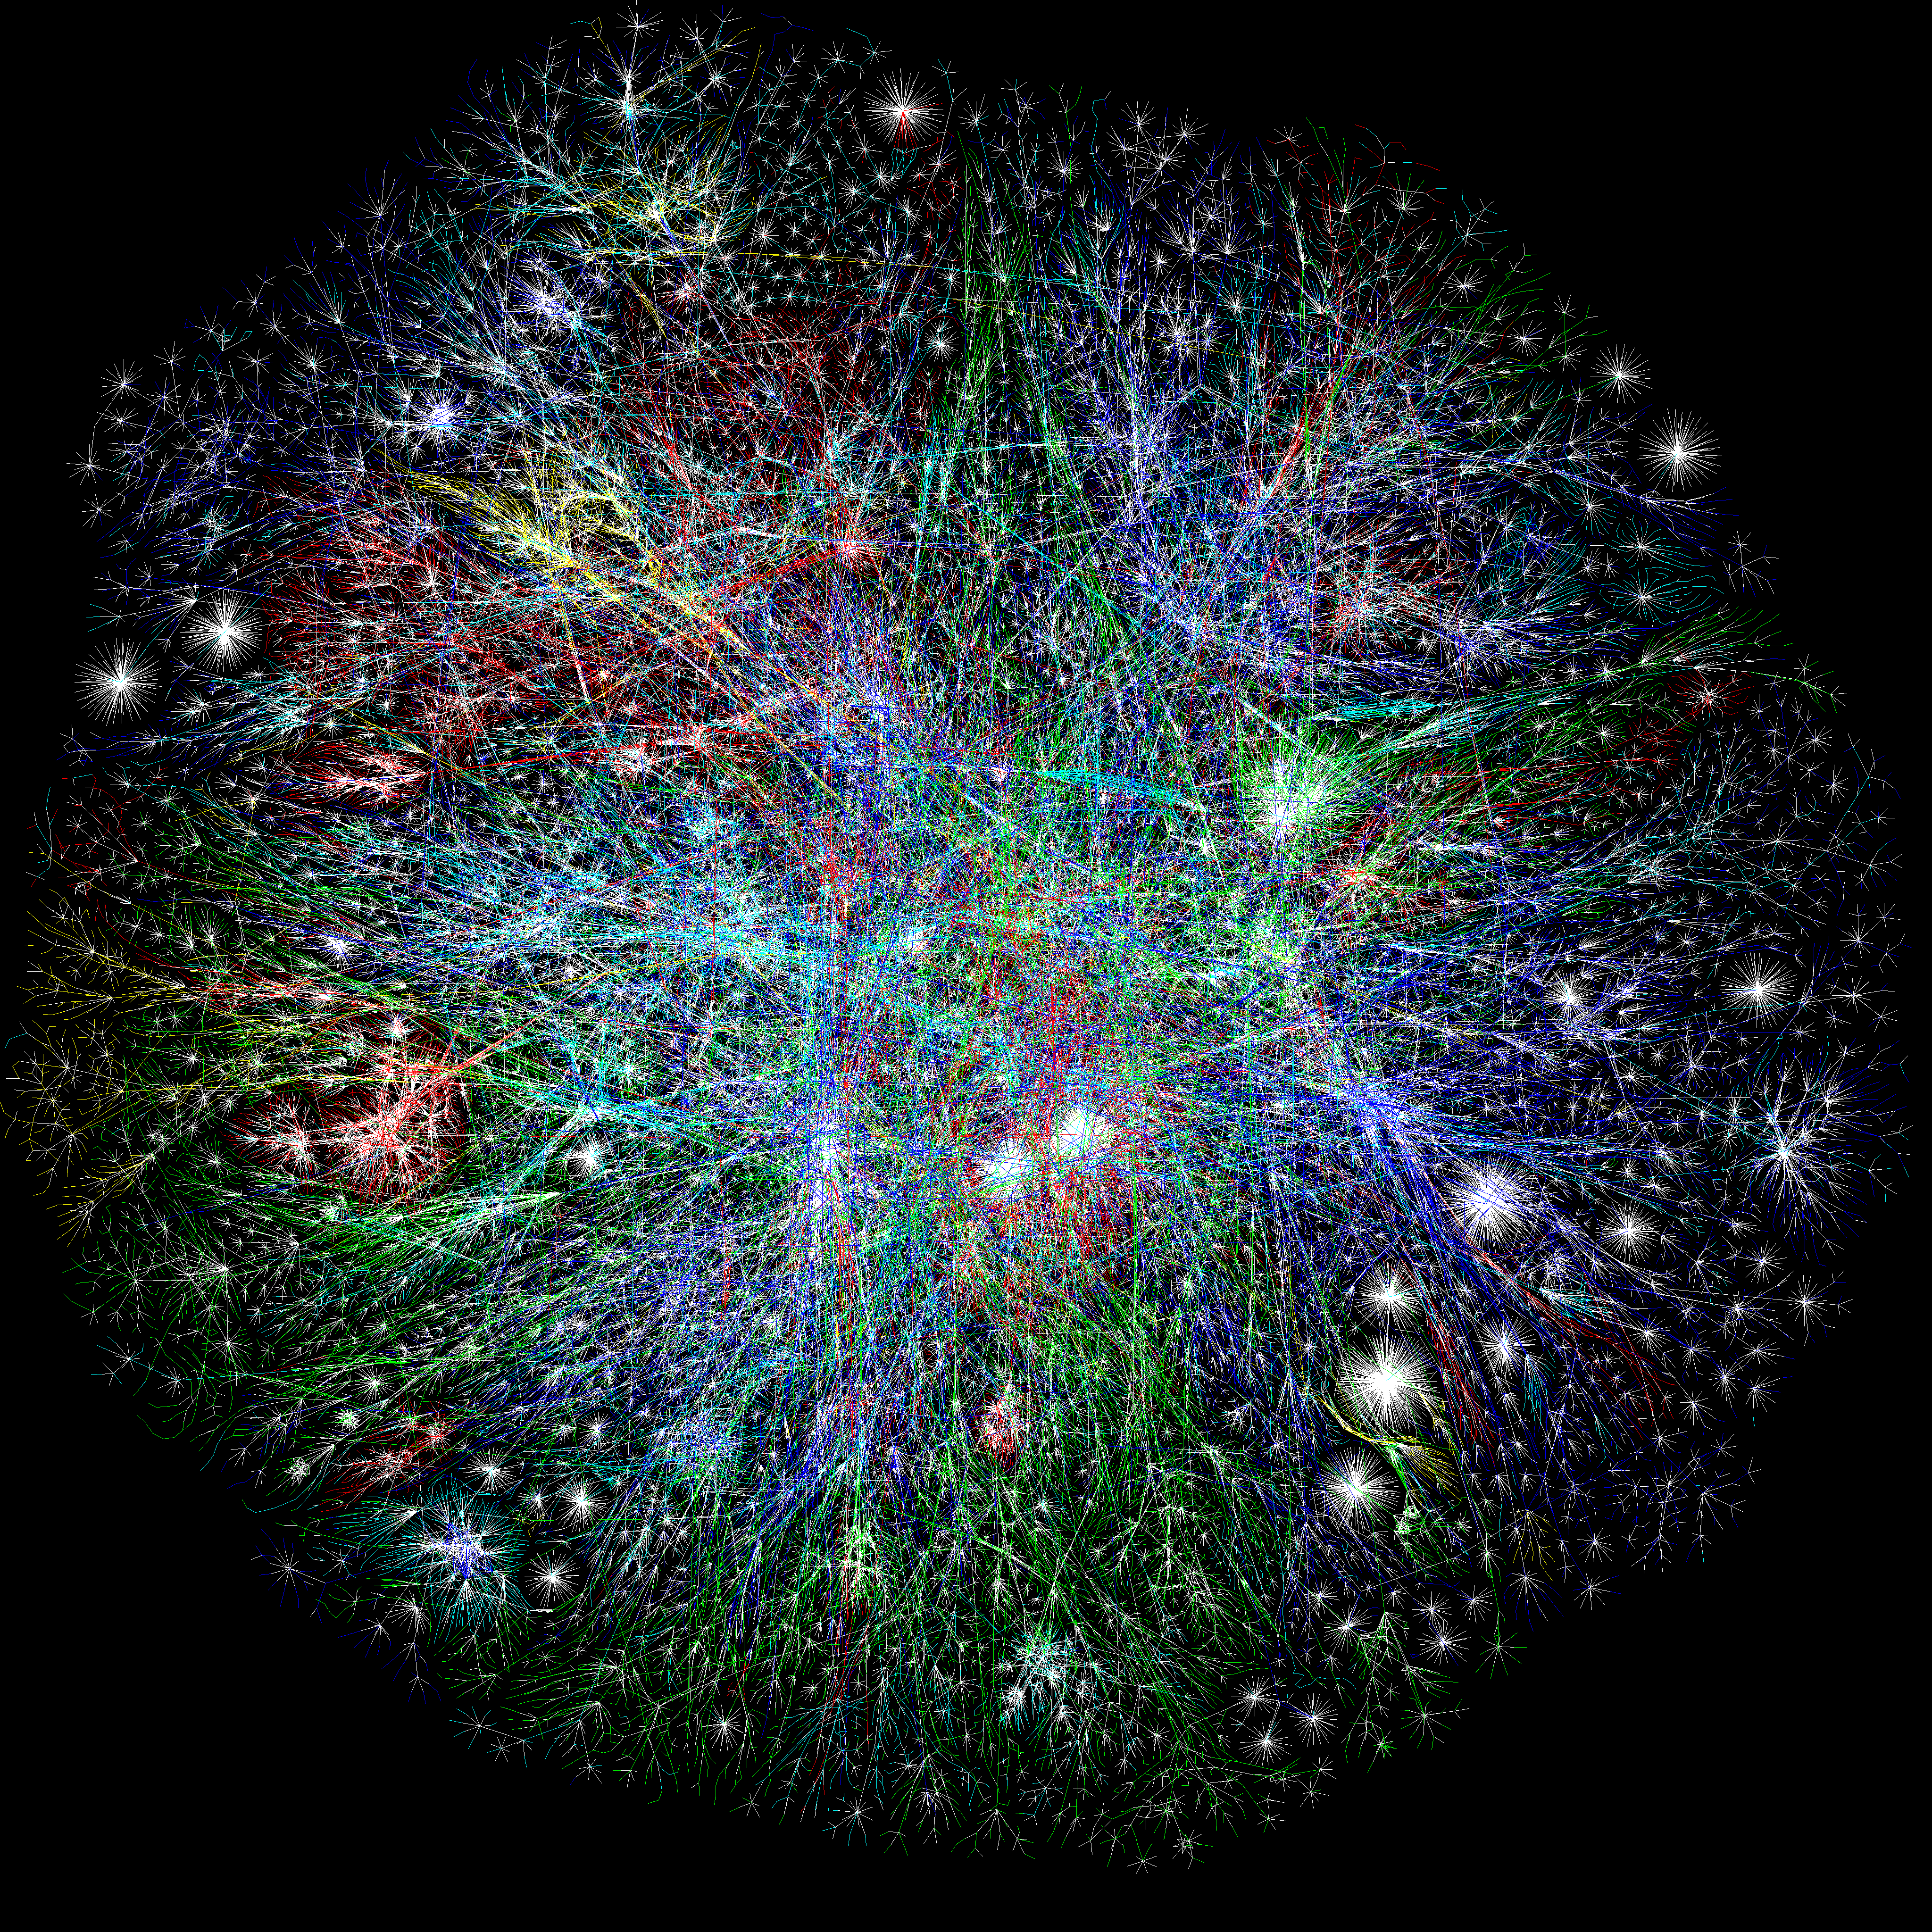
\includegraphics[width = \paperwidth]{InternetGraph.png}}
\setbeamertemplate{blocks}[rounded][shadow=false]
\begin{frame}
  \frametitle{Pagerank : motivation}
  \begin{block}{Where to start searching the web}
  \begin{itemize}
    \item How to find one's way through the millions of webpages of the web?
    \item Access webpage only from a URL or an hyperlink
    \end{itemize}
  \end{block}
\end{frame}


\setbeamertemplate{background canvas}{}
\setbeamertemplate{blocks}[rounded][shadow=false]
\begin{frame}{Search engines}
  \begin{block}{Answer}
    \begin{itemize}
      \item Use of search engines
      \item Centralization : you only need to know the address of the search engine
      \item New challenge : order pages by relevancy
    \end{itemize}
  \end{block}
  \begin{figure}
    \centering
    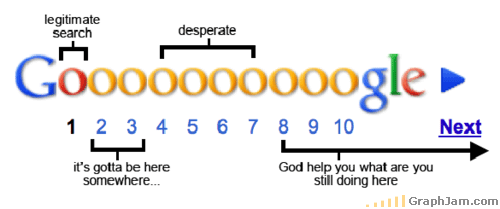
\includegraphics[width = 8cm]{google-search-result-pages.png}
  \end{figure}

\end{frame}


\begin{frame}{Early search engines}
  \begin{block}{Naive ordering}
    \begin{itemize}
      \item Early search engine's simply listed the terms in each page, making it easy to fool the search engine using \textbf{term spam}

    \end{itemize}
  \end{block}
  \begin{figure}
    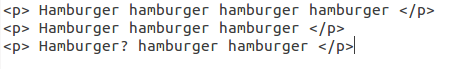
\includegraphics[width = 10cm]{termspam.png}
  \end{figure}
  \begin{block}{Pagerank}
    \begin{itemize}
      \item The game changed with Google's arrival and the use of this algorithm in search engines
    \end{itemize}
  \end{block}
\end{frame}

\begin{frame}{PageRank : a measure of importance}
\begin{columns}
    \begin{column}{5cm}
      \begin{block}{The internet as a graph}
        Directed graph $\mathcal{G}$, pages are nodes and there is an arc from node p1 to node p2 if there is at least one link from p1 to p2
      \end{block}
      %TODO : Successeurs predecesseurs
    \end{column}
    \begin{column}{5cm}
      \begin{figure}[r]
        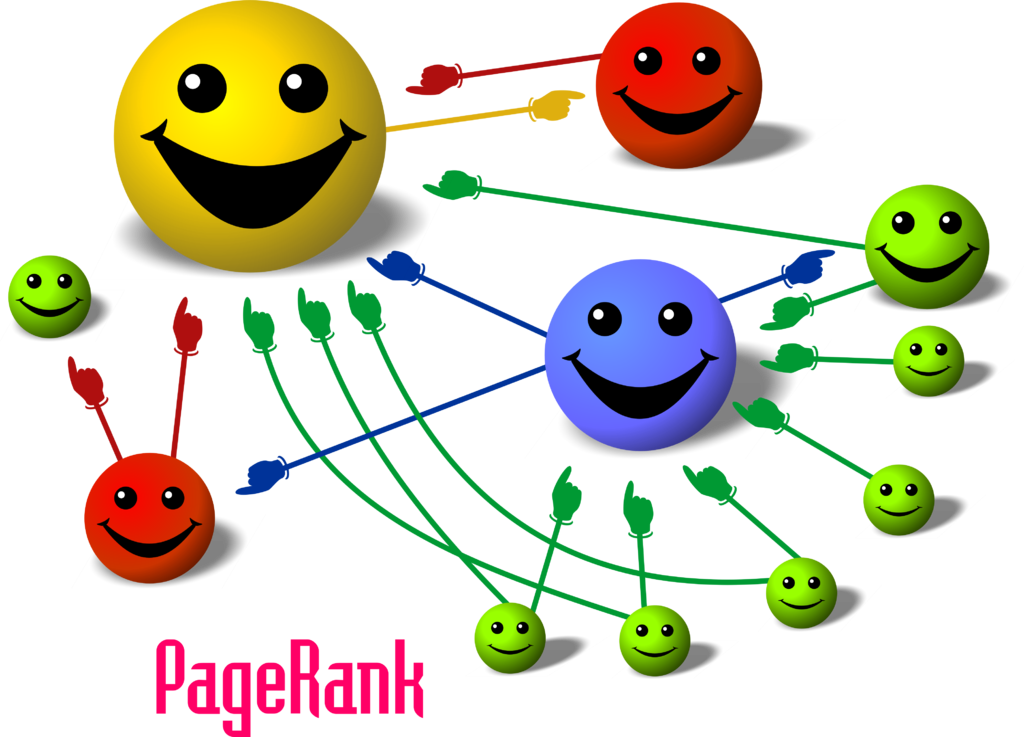
\includegraphics[width =4.5cm]{PageRank-hi-res.png}
      \end{figure}
    \end{column}
  \end{columns}
\begin{block}{Importance of a page}
\begin{itemize}
\item A page is important if other important pages are its predecessors
\item Webmasters vote for the best pages by placing links to useful websites on their own sites
\end{itemize}
\end{block}
\end{frame}


\setbeamertemplate{background canvas}{
\includegraphics[height = \paperheight]{surfer.png}}
\setbeamertemplate{blocks}[rounded][shadow=false]
\addtobeamertemplate{block begin}{\pgfsetfillopacity{0.7}}{\pgfsetfillopacity{1}}
\begin{frame}[allowframebreaks]{The random web surfer model}
  \begin{block}{The random surfer}
    \begin{itemize}
      \item Is travelling the web randomly, by following out-links from the webpages he visits
      \item Given that the surfer is on some page p, each out-link of p has an equal probability to be followed  
    \end{itemize}
    $\rightarrow$ Has been proved to work empirically
  \end{block}
  \begin{definition}
  The idealized PageRank of a certain page p is the likelihood of a random surfer to be at page p after following an infinity of links
  
  \end{definition}
\end{frame}

\setbeamertemplate{background canvas}{}
\setbeamertemplate{blocks}[shadow=true]
\begin{frame}{The random web surfer model : example}
      \begin{figure}
      \centering
        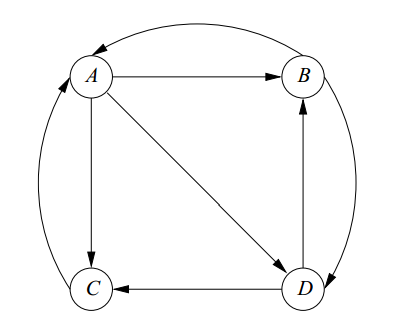
\includegraphics[width = 5cm]{graph1.png}
      \end{figure}
\end{frame}

\begin{frame}{The random surfer web model}
\begin{block}{Probability of being at a certain page p}
\begin{itemize}
\item Let $p$ be a node of the web graph, $pos_i$ the location of the random surfer at the $i+1^{th}$ step of the surfer
$$ P(pos_{i+1}=p) = \sum_{n_i\in V} P(pos_{i+1}=p|pos_{i}=n_i)  P(pos_i = n_i)$$
\end{itemize}
\end{block}
\begin{columns}
\centering
\begin{column}{0.5\paperwidth}
\begin{block}{Probability vector}
\begin{itemize}
\item $ v_i = 
\begin{pmatrix}
P(pos_i = p_1) \\
\vdots \\
P(pos_i = p_n)
\end{pmatrix}
$
\item Random walk is modelled by the iteration $v_{i+1} = M v_i$
\end{itemize}

\end{block}
\end{column}
\begin{column}{0.4\paperwidth}
$$M = \begin{pmatrix}
0 & \frac{1}{2} & 1 & 0 \\
\frac{1}{3} & 0 & 0 & \frac{1}{2} \\
\frac{1}{3} & 0 & 0 & \frac{1}{2} \\
\frac{1}{3} & \frac{1}{2} & 0 & 0 \\
\end{pmatrix}$$
\end{column}
\end{columns}
\end{frame}

\begin{frame}{Definition of PageRank}
  \begin{definition}
    \begin{itemize}
      \item A function that assigns a real number to each page
	\item It is the limiting stationnary distribution of the location of the random surfer
    \end{itemize}
    $$Pgrk(\mathcal{G}) = v \:s.t.\: v=Mv $$
  \end{definition}
  \begin{algorithm}[H]
    \KwData{Oriented graphe $ G$, start vector $v_0 = \begin{pmatrix} 1/n \\ \vdots \\ 1/n \end{pmatrix}$}
    \KwResult{PageRank $v$}
    $v_1 = Mv_0$\;
    $i=0$\;
    \While{$||v_{i+1}-v_{i}||>tol$}{
      $v_{i+1} = M v_i$\;
      $i++$\;
    }
    $v = v_{i}$\;
    \caption{PageRank}
  \end{algorithm}
\end{frame}

\begin{frame}{Remarks}
\begin{itemize}
\item This is the power method for eigenvalues
\item In this case, the sum of the components of each column is 1, no need to norm the iterates
\item We can chose any initial vector $v_0$ as long as the sum of its components is 1 and it has no zero component, because then $(v_0|v)$ is never zero
\item This will influe on convergence speed
\item For the world wide web : 50-75 iterations are generally needed
\end{itemize}
\end{frame}

\begin{frame}{Convergence and limiting cases}
\begin{block}{Convergence}
Convergence and unicity are guaranteed if the graph is strongly connected
\end{block}
\begin{block}{How to deal with particular structures}
Non-SCC graphs : 
\begin{itemize}
\item Dead-ends
\item Spider traps
\item ...
\end{itemize}
\end{block}
\end{frame}


\begin{frame}{Power iteration}
  Let $A$ be a square matrix with eigenvalues $|\lambda_1| \geq |\lambda_2| \geq \cdots |\lambda_n|$ and
  $v_k$ such that
  \begin{align*}
    v_{k+1} & = \frac{Av_k}{\|Av_k\|}\\
    v_0 & = \sum_{i=1}^n \alpha_i x_i\\
    v_k & = \sum_{i=1}^n \alpha_i \lambda_i^k x_i\\
        & = \lambda_1^k \sum_{i=1}^n \alpha_i \left(\frac{\lambda_i}{\lambda_1}\right)^k x_i
  \end{align*}
  where for simplicity all eigenvalues are simple.


  If $|\lambda_1| > |\lambda_2|$, $\exists \phi_k$ such that $e^{i\phi_k}v_k$ converges (e.g. $\lambda_1 = i$).

  If $\lambda_k$ is simple, it is unique.
  Else it depends on the projection of $v_0$ on the space of eigenvectors of $\lambda_1$.
\end{frame}

\begin{frame}{Strongly Connected Components}
  \vspace{-.5cm}
  \begin{columns}
    \begin{column}{0.4\textwidth}
      \begin{itemize}
        \item Strongly Connected Components (SCC) : $\exists$ path $u \to v$ $\forall u,v \in \mathsf{SCC}$.
        \item Component graph is a Directed Acyclic Graph (DAG).
        \item Computed on $\bigoh(|V| + |E|)$ with DFS (Tarjan or CLRS).
          They also toposort the DAG.
      \end{itemize}
    \end{column}
    \begin{column}{0.6\textwidth}
      \begin{center}
        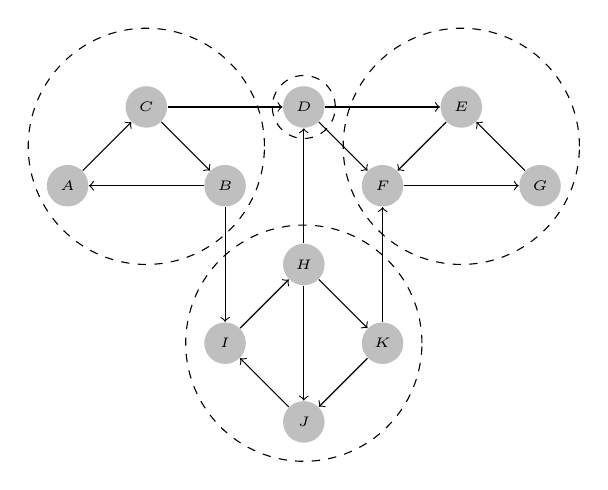
\begin{tikzpicture}
          \node[vertex] at (0, 0) (A) {\tiny $A$};
          \node[vertex] at (2, 0) (B) {\tiny $B$};
          \node[vertex] at (1, 1) (C) {\tiny $C$};
          \node[vertex] at (3, 1) (D) {\tiny $D$};
          \node[vertex] at (5, 1) (E) {\tiny $E$};
          \node[vertex] at (4, 0) (F) {\tiny $F$};
          \node[vertex] at (6, 0) (G) {\tiny $G$};
          \node[vertex] at (3, -1) (H) {\tiny $H$};
          \node[vertex] at (2, -2) (I) {\tiny $I$};
          \node[vertex] at (3, -3) (J) {\tiny $J$};
          \node[vertex] at (4, -2) (K) {\tiny $K$};

          \draw[->] (A) edge (C);
          \draw[->] (C) edge (B);
          \draw[->] (B) edge (A);
          \draw[->] (C) edge (D);
          \draw[->] (D) edge (E);
          \draw[->] (D) edge (F);
          \draw[->] (E) edge (F);
          \draw[->] (F) edge (G);
          \draw[->] (B) edge (I);
          \draw[->] (K) edge (F);
          \draw[->] (I) edge (H);
          \draw[->] (H) edge (K);
          \draw[->] (K) edge (J);
          \draw[->] (J) edge (I);
          \draw[->] (H) edge (J);
          \draw[->] (H) edge (D);
          \draw[->] (G) edge (E);

          \draw[dashed] (1, 0.5) circle (1.5);
          \draw[dashed] (5, 0.5) circle (1.5);
          \draw[dashed] (3, -2) circle (1.5);
          \draw[dashed] (3, 1) circle (0.4);
        \end{tikzpicture}
      \end{center}
    \end{column}
  \end{columns}
  \begin{center}
    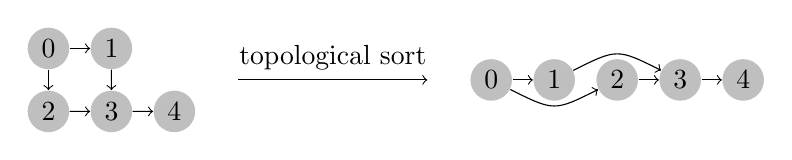
\begin{tikzpicture}[scale = 0.8]
      \begin{scope}[xshift=-100]
        \node[vertex] (n0) at (0, 0) {0};
        \node[vertex] (n1) at (1, 0) {1};
        \node[vertex] (n2) at (0, -1) {2};
        \node[vertex] (n3) at (1, -1) {3};
        \node[vertex] (n4) at (2, -1) {4};
        \draw[->] (n0) -- (n1);
        \draw[->] (n0) -- (n2);
        \draw[->] (n2) -- (n3);
        \draw[->] (n1) -- (n3);
        \draw[->] (n3) -- (n4);
      \end{scope}

      \begin{scope}
        \draw[->, anchor=south] (-0.5,-0.5) -- (1,-0.5) node{topological sort} -- (2.5,-0.5);
      \end{scope}

      \begin{scope}[xshift=100]
        \node[vertex] (n0) at (0, -0.5) {0};
        \node[vertex] (n1) at (1, -0.5) {1};
        \node[vertex] (n2) at (2, -0.5) {2};
        \node[vertex] (n3) at (3, -0.5) {3};
        \node[vertex] (n4) at (4, -0.5) {4};
        \draw[->] (n0) -- (n1);
        \draw[->] (n0) .. controls (1,-1) .. (n2);
        \draw[->] (n2) -- (n3);
        \draw[->] (n1) .. controls (2,0) .. (n3);
        \draw[->] (n3) -- (n4);
      \end{scope}
    \end{tikzpicture}
  \end{center}
\end{frame}

\begin{frame}{Actual Web graph}
  \begin{columns}
    \begin{column}{0.5\textwidth}
      \begin{itemize}
        \item One BIG SCC: ``Main SCC''.
        \item Tendrils out, Disconnected Components and Out Components:
          have at least one SCC with no arcs out.
          \begin{description}
            \item[dead end] only 1 page in the SCC.
            \item[spider strap] SCC with more than 1 page.
          \end{description}
        \item If Out Components is empty, Main SCC is a spider trap.
      \end{itemize}
    \end{column}
    \begin{column}{0.5\textwidth}
      \begin{figure}
        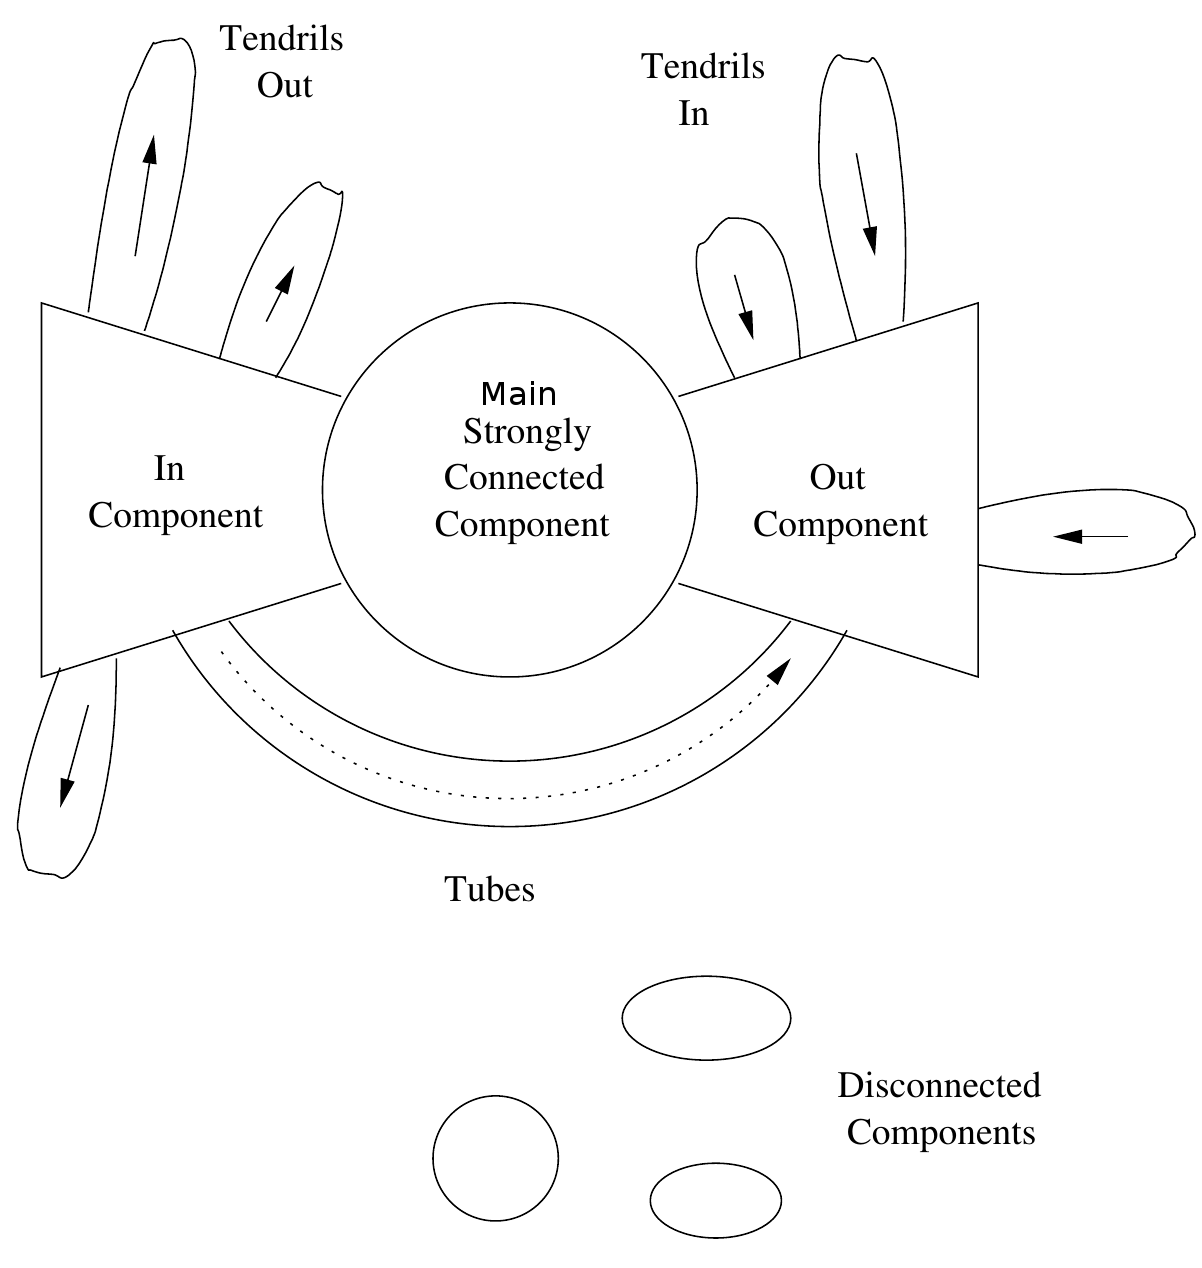
\includegraphics[trim=.5cm 0cm .2cm 0cm,clip,width=\linewidth]{web-graph.png}
        \caption{The ``bowtie'' picture of the Web \cite[p.~187]{leskovec2014mining} (modified).}
        \label{fig:web-graph}
      \end{figure}
    \end{column}
  \end{columns}
\end{frame}

\begin{frame}{Dead ends}
  Links to dead ends are called Dangling links.
  \begin{block}{Original Google solution \cite[p.~6]{ilprints422}}
    They can also be undownloaded pages (51 million URL not not downloaded yet in 1999 at Google).

    \begin{itemize}
      \item Remove dead ends and corresponding Dangling links before computing $A$.
      \item Compute $A$ and PageRank
      \item ``After all the PageRanks are calculated, they can be added back in, without affecting things significantly''
        \cite[p.~6]{ilprints422}.
    \end{itemize}
  \end{block}
  \begin{center}
    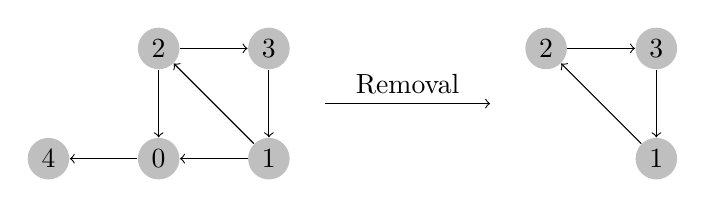
\begin{tikzpicture}[scale = 0.7]
      \begin{scope}[xshift=-100]
        \node[vertex] (n0) at (0, -1) {0};
        \node[vertex] (n1) at (2, -1) {1};
        \node[vertex] (n2) at (0, 1) {2};
        \node[vertex] (n3) at (2, 1) {3};
        \node[vertex] (n4) at (-2, -1) {4};
        \draw[->] (n1) -- (n2);
        \draw[->] (n2) -- (n3);
        \draw[->] (n3) -- (n1);
        \draw[->] (n2) -- (n0);
        \draw[->] (n1) -- (n0);
        \draw[->] (n0) -- (n4);
      \end{scope}

      \begin{scope}
        \draw[->, anchor=south] (-0.5,0) -- (1,0) node{Removal} -- (2.5,0);
      \end{scope}

      \begin{scope}[xshift=100]
        \node[vertex] (n1) at (2, -1) {1};
        \node[vertex] (n2) at (0, 1) {2};
        \node[vertex] (n3) at (2, 1) {3};
        \draw[->] (n1) -- (n2);
        \draw[->] (n2) -- (n3);
        \draw[->] (n3) -- (n1);
      \end{scope}
    \end{tikzpicture}
  \end{center}
\end{frame}

\begin{frame}{Add an Infinite Improbability Drive on them}
  \begin{center}
    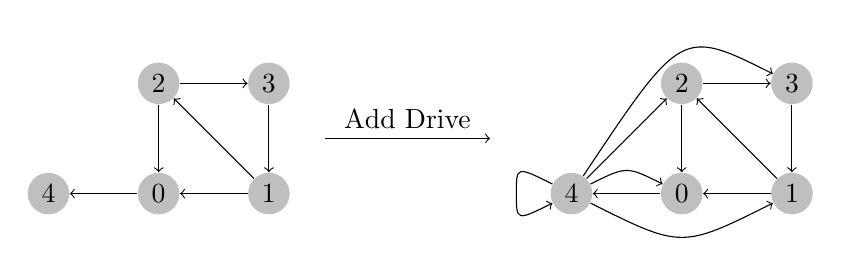
\begin{tikzpicture}[scale = 0.7]
      \begin{scope}[xshift=-100]
        \node[vertex] (n0) at (0, -1) {0};
        \node[vertex] (n1) at (2, -1) {1};
        \node[vertex] (n2) at (0, 1) {2};
        \node[vertex] (n3) at (2, 1) {3};
        \node[vertex] (n4) at (-2, -1) {4};
        \draw[->] (n1) -- (n2);
        \draw[->] (n2) -- (n3);
        \draw[->] (n3) -- (n1);
        \draw[->] (n2) -- (n0);
        \draw[->] (n1) -- (n0);
        \draw[->] (n0) -- (n4);
      \end{scope}

      \begin{scope}
        \draw[->, anchor=south] (-0.5,0) -- (1,0) node{Add Drive} -- (2.5,0);
      \end{scope}

      \begin{scope}[xshift=170]
        \node[vertex] (n0) at (0, -1) {0};
        \node[vertex] (n1) at (2, -1) {1};
        \node[vertex] (n2) at (0, 1) {2};
        \node[vertex] (n3) at (2, 1) {3};
        \node[vertex] (n4) at (-2, -1) {4};
        \draw[->] (n1) -- (n2);
        \draw[->] (n2) -- (n3);
        \draw[->] (n3) -- (n1);
        \draw[->] (n2) -- (n0);
        \draw[->] (n1) -- (n0);
        \draw[->] (n0) -- (n4);
        \draw[->] (n4) .. controls (-1,-.5) ..  (n0);
        \draw[->] (n4) .. controls (0,-2) ..  (n1);
        \draw[->] (n4) --  (n2);
        \draw[->] (n4) .. controls (0,2) ..  (n3);
        \draw[->] (n4) .. controls (-3,-.5) .. (-3,-1) ..  controls (-3,-1.5) .. (n4);
      \end{scope}
    \end{tikzpicture}
  \end{center}
  \[
    \begin{pmatrix}
      0 & 1/2 & 1/2 & 0 & 0\\
      0 & 0   & 0   & 1 & 0\\
      0 & 1/2 & 0   & 0 & 0\\
      0 & 0   & 1/2 & 0 & 0\\
      1 & 0   & 0   & 0 & 0
    \end{pmatrix}
    \to
    \begin{pmatrix}
      0 & 1/2 & 1/2 & 0 & 1/5\\
      0 & 0 & 0   & 1 & 1/5\\
      0 & 1/2 & 0   & 0 & 1/5\\
      0 & 0 & 1/2 & 0 & 1/5\\
      1 & 0 & 0   & 0 & 1/5
    \end{pmatrix}
  \]
\end{frame}

\begin{frame}[allowframebreaks]{Perron-Frobenius}
  \begin{block}{Irreducible matrix}
    Let $G_A$ be a directed graph where $(i,j) \in E$ iff $A_{ij} > 0$.
    $A$ is irreducible iff $G_A$ is strongly connected.

    In this case, the period of $A$ is the GCD of the lengths of the closed directed paths
    of $G_A$ or the number $m$ such that $(A^m)_{ii} > 0$ $\forall i$
    (which will be at the same time for each $i$ since $A$ is irreducible~\cite{kitchens1998symbolic}).
  \end{block}
  \begin{block}{Perron-Frobenius}
    \begin{itemize}
      \item If $A_{ij} \geq 0$ $\forall i,j$, $A$ is irreducible with period $h$.
        There is $h$ eigenvalues s.t. $|\lambda_i| = \rho(A)$.
        One of them is positive real and its has an eigenvector with only positive real components.
        They are simple (i.e. $m_a(\lambda_i) = 1$).
        \[ \min_i \sum_j A_{ij} \leq \rho(A) \leq \max_i \sum_j A_{ij} (= 1 \text{ in our case}) \]
      \item If $A_{ij} > 0$ $\forall i,j$, everything above is true with $h=1$ since it is irreducible.
        There is one \emph{simple} positive real eigenvalue $\lambda$ with a eigenvector with only positive real components
        such that $|\lambda| > |\lambda_i|$ for all $\lambda_i \neq \lambda$.
    \end{itemize}
    Since an eigenvector has \emph{positive} real values, if the the $\min \neq \max$,
    \[ \min_i \sum_j A_{ij} < \rho(A) < \max_i \sum_j A_{ij}. \]
  \end{block}
\end{frame}

\begin{frame}[allowframebreaks]{Convergence of PageRank}
  \begin{block}{Sufficient condition from the book}
    ``If the graph is \emph{strongly connected} and has no \emph{dead end}, $v$ converge to a limit such that $v = Mv$''
    \cite[p.~185]{leskovec2014mining}.
  \end{block}
  \begin{block}{Actual not so sufficient condition}
    ``In the Main SCC (everything else empty or removed), $v$ \emph{might} converge to a limit such that $v = Mv$''.
  \end{block}
  Since $h$ is not necessarily one, we don't have the convergence (e.g. bipartie graphs where $h=2$).
  \framebreak

  Page rank of all pages is 0 except for pages in spider trap.
  \begin{proof}
    We have a DAG of SCC so there exists a SCC with no in arcs, its pages have indices in $I$.
    Let's consider the iteration with $B = A_{I,I}$ and $w=v_I$.
    If it is not a spider trap, $\max_i \sum_j A_{ij} < 1$.
    Since $B$ is SC, by Perron-Frobenius,
    \[ 0 < \rho(B) < 1 \]
    $w_k$ converges therefore to 0.

    ``Remove'' (needs $\epsilon$ game here) this SCC and iterate.
  \end{proof}
\end{frame}

\begin{frame}{Non-convergent example 1}
  \begin{columns}
    \begin{column}{0.4\textwidth}
      $h=4$
      \[ v_k = \alpha_1 x_1 + \alpha_2 i^k x_2 + \alpha_3 (-1)^k x_3 + \alpha_4 (-i)^k x_4. \]
      With $v_0 = x_1/4 + x_2/8 + x_4/8$:
      \[
        \begin{pmatrix}
          1/2\\
          1/4\\
          0\\
          1/4
        \end{pmatrix},
        \begin{pmatrix}
          1/4\\
          1/2\\
          1/4\\
          0
        \end{pmatrix},
        \begin{pmatrix}
          0\\
          1/4\\
          1/2\\
          1/4
        \end{pmatrix},
        \begin{pmatrix}
          1/4\\
          0\\
          1/4\\
          1/2
        \end{pmatrix},\ldots
      \]
      With classical $v_0$ ($= x_1/4$ here):
      \[
        \begin{pmatrix}
          1/4\\
          1/4\\
          1/4\\
          1/4
        \end{pmatrix},
        \begin{pmatrix}
          1/4\\
          1/4\\
          1/4\\
          1/4
        \end{pmatrix},\ldots
      \]
    \end{column}
    \begin{column}{0.6\textwidth}
      \begin{center}
        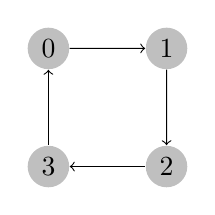
\begin{tikzpicture}[scale = 1.5]
          \node[vertex] (n0) at (0, 1) {0};
          \node[vertex] (n1) at (1, 1) {1};
          \node[vertex] (n2) at (1, 0) {2};
          \node[vertex] (n3) at (0, 0) {3};
          \draw[->] (n0) -- (n1);
          \draw[->] (n1) -- (n2);
          \draw[->] (n2) -- (n3);
          \draw[->] (n3) -- (n0);
        \end{tikzpicture}
      \end{center}
      \[
        A =
        \begin{pmatrix}
          0 & 0 & 0 & 1\\
          1 & 0 & 0 & 0\\
          0 & 1 & 0 & 0\\
          0 & 0 & 1 & 0
        \end{pmatrix}
      \]
      \[
        1,
        \begin{pmatrix}1\\1\\1\\1
        \end{pmatrix};
        i,
        \begin{pmatrix}1\\i\\-1\\-i
        \end{pmatrix};
        -1,
        \begin{pmatrix}1\\-1\\1\\-1
        \end{pmatrix};
        -i,
        \begin{pmatrix}1\\-i\\-1\\i
        \end{pmatrix}.
      \]
    \end{column}
  \end{columns}
\end{frame}

\begin{frame}[allowframebreaks]{Non-convergent example 2}
  \begin{center}
    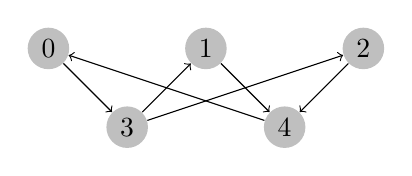
\begin{tikzpicture}[scale = .5]
      \node[vertex] (n0) at (-4, 1) {0};
      \node[vertex] (n1) at (0, 1) {1};
      \node[vertex] (n2) at (4, 1) {2};
      \node[vertex] (n3) at (-2, -1) {3};
      \node[vertex] (n4) at ( 2, -1) {4};
      \draw[->] (n0) -- (n3);
      \draw[->] (n1) -- (n4);
      \draw[->] (n2) -- (n4);
      \draw[->] (n3) -- (n1);
      \draw[->] (n3) -- (n2);
      \draw[->] (n4) -- (n0);
    \end{tikzpicture}
  \end{center}
  \[
    A =
    \begin{pmatrix}
      0 & 0 & 0 &   0 & 1\\
      0 & 0 & 0 & 1/2 & 0\\
      0 & 0 & 0 & 1/2 & 0\\
      1 & 0 & 0 & 0   & 0\\
      0 & 1 & 1 & 0   & 0
    \end{pmatrix}
  \]
  \[
    1,
    \begin{pmatrix}1/4\\1/8\\1/8\\1/4\\1/4
    \end{pmatrix};
    i,
    \begin{pmatrix}-i\\i/2\\i/2\\-1\\1
    \end{pmatrix};
    -1,
    \begin{pmatrix}-1\\-1/2\\-1/2\\1\\1
    \end{pmatrix};
    -i,
    \begin{pmatrix}i\\-i/2\\-i/2\\-1\\1
    \end{pmatrix};
    0,
    \begin{pmatrix}0\\1\\-1\\0\\0
    \end{pmatrix}.
  \]
  \framebreak

  $h=4$
  \[
    v_k = \alpha_1 x_1 + \alpha_2 i^k x_2 + \alpha_3 (-1)^k x_3 + \alpha_4 (-i)^k x_4.
  \]
  With classical $v_0$ ($= x_1-x_2i/20-x_3/20+x_4i/20$ here):
  \[
    \begin{pmatrix}
      0.2\\
      0.2\\
      0.2\\
      0.2\\
      0.2
    \end{pmatrix},
    \begin{pmatrix}
      0.2\\
      0.1\\
      0.1\\
      0.2\\
      0.4
    \end{pmatrix},
    \begin{pmatrix}
      0.4\\
      0.1\\
      0.1\\
      0.2\\
      0.2
    \end{pmatrix},
    \begin{pmatrix}
      0.2\\
      0.1\\
      0.1\\
      0.4\\
      0.2
    \end{pmatrix},
    \begin{pmatrix}
      0.2\\
      0.2\\
      0.2\\
      0.2\\
      0.2
    \end{pmatrix}
    ,\ldots
  \]

\end{frame}

\begin{frame}[allowframebreaks]{Solution 1 : pruning}
  \begin{algorithm}[H]
    \KwData{DAG $G$}
    \KwResult{Pruned $G$}
    \While{$G$ has a node $u$ with no arcs out}{
      remove incoming arcs of $u$\;
      remove $u$\;
    }
    \caption{Pruning a DAG}
  \end{algorithm}
  \begin{center}
    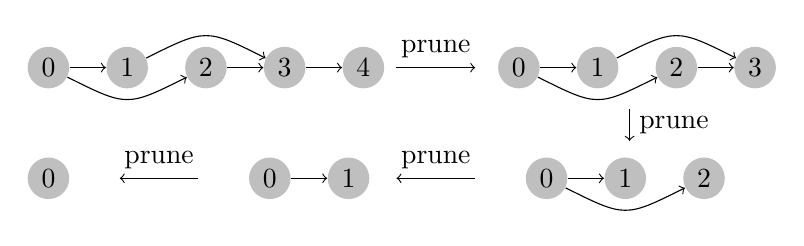
\begin{tikzpicture}
      \begin{scope}[xshift=-100]
        \node[vertex] (n0) at (0, -0.5) {0};
        \node[vertex] (n1) at (1, -0.5) {1};
        \node[vertex] (n2) at (2, -0.5) {2};
        \node[vertex] (n3) at (3, -0.5) {3};
        \node[vertex] (n4) at (4, -0.5) {4};
        \draw[->] (n0) -- (n1);
        \draw[->] (n0) .. controls (1,-1) .. (n2);
        \draw[->] (n2) -- (n3);
        \draw[->] (n1) .. controls (2,0) .. (n3);
        \draw[->] (n3) -- (n4);
      \end{scope}
      \begin{scope}[xshift=40]
        \draw[->, anchor=south] (-0.5,-0.5) -- (0,-0.5) node{prune} -- (0.5,-0.5);
      \end{scope}
      \begin{scope}[xshift=70]
        \node[vertex] (n0) at (0, -0.5) {0};
        \node[vertex] (n1) at (1, -0.5) {1};
        \node[vertex] (n2) at (2, -0.5) {2};
        \node[vertex] (n3) at (3, -0.5) {3};
        \draw[->] (n0) -- (n1);
        \draw[->] (n0) .. controls (1,-1) .. (n2);
        \draw[->] (n2) -- (n3);
        \draw[->] (n1) .. controls (2,0) .. (n3);
      \end{scope}
      \begin{scope}[xshift=110,yshift=-35]
        \draw[->, anchor=west] (0,0.2) -- (0,0) node{prune} -- (0,-0.2);
      \end{scope}
      \begin{scope}[xshift=80,yshift=-40]
        \node[vertex] (n0) at (0, -0.5) {0};
        \node[vertex] (n1) at (1, -0.5) {1};
        \node[vertex] (n2) at (2, -0.5) {2};
        \draw[->] (n0) -- (n1);
        \draw[->] (n0) .. controls (1,-1) .. (n2);
      \end{scope}
      \begin{scope}[xshift=40,yshift=-40]
        \draw[->, anchor=south] (0.5,-0.5) -- (0,-0.5) node{prune} -- (-0.5,-0.5);
      \end{scope}
      \begin{scope}[xshift=-20,yshift=-40]
        \node[vertex] (n0) at (0, -0.5) {0};
        \node[vertex] (n1) at (1, -0.5) {1};
        \draw[->] (n0) -- (n1);
      \end{scope}
      \begin{scope}[xshift=-60,yshift=-40]
        \draw[->, anchor=south] (0.5,-0.5) -- (0,-0.5) node{prune} -- (-0.5,-0.5);
      \end{scope}
      \begin{scope}[xshift=-100,yshift=-40]
        \node[vertex] (n0) at (0, -0.5) {0};
      \end{scope}
    \end{tikzpicture}
  \end{center}
  In our case, we need to keep the Main SCC.
  $\bigoh(|V| + |E|)$ using the toposort order.

  \framebreak

  \begin{columns}
    \begin{column}{0.5\textwidth}
      \begin{block}{Interpretation}
        We only consider pages in the Main SCC or a page that \emph{indirectly} links to a page in the Main SCC.
      \end{block}
      Every node in the In Component will have PageRank 0 so we can remove it too for optimization.

      % TODO still a problem, conv
    \end{column}
    \begin{column}{0.5\textwidth}
      \begin{figure}
        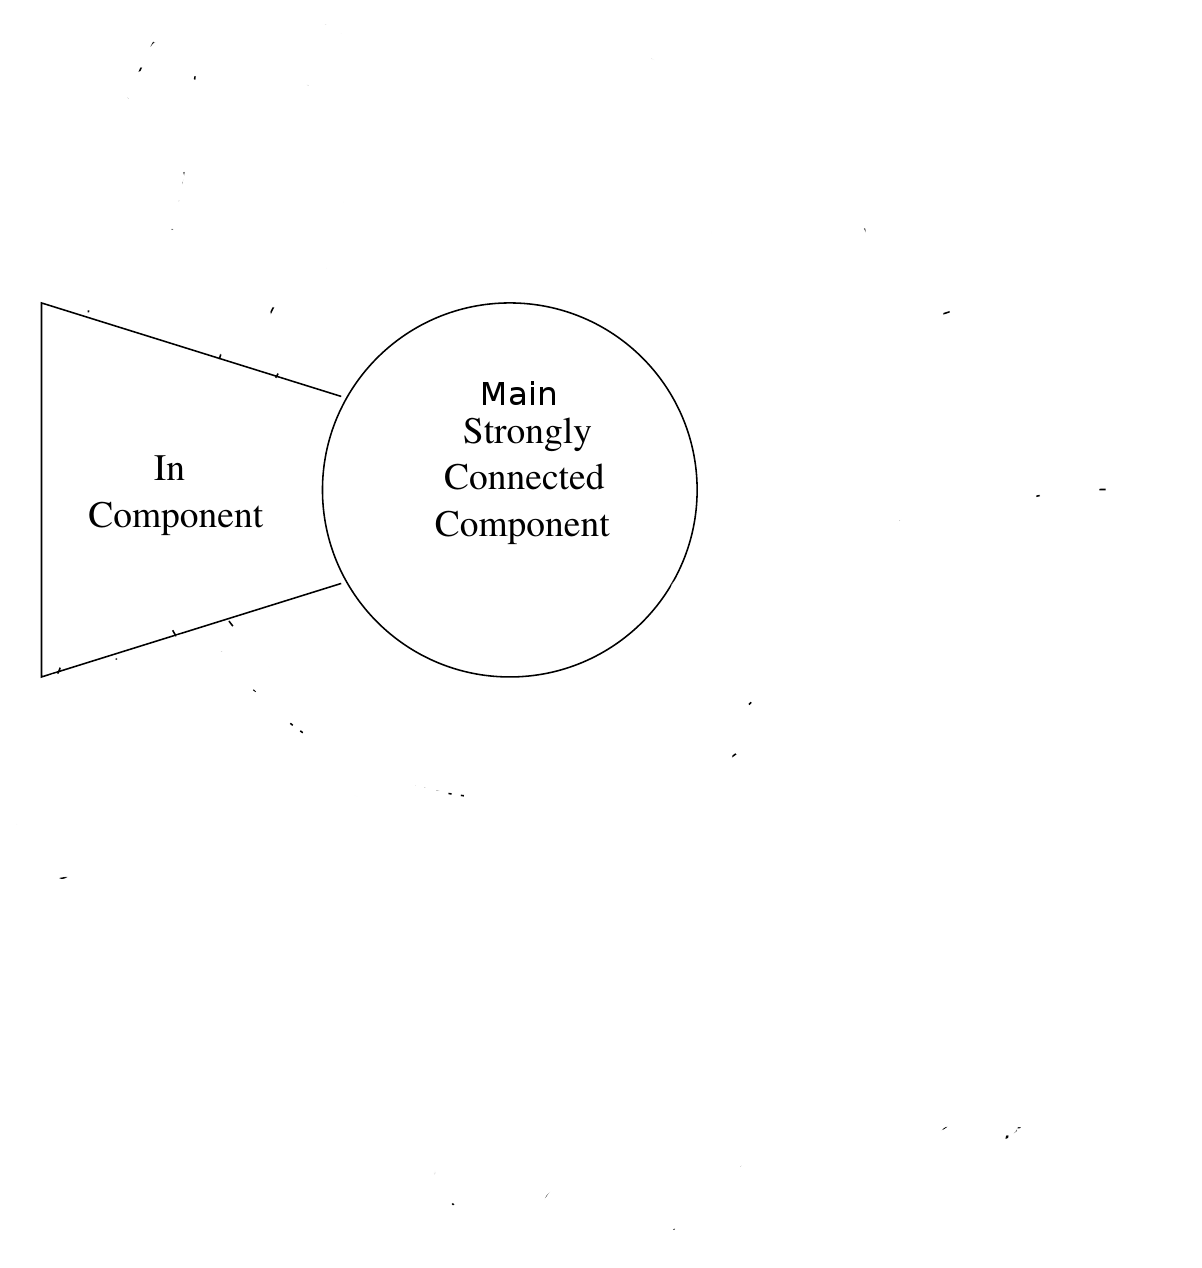
\includegraphics[trim=.5cm 0cm .2cm 0cm,clip,width=\linewidth]{web-graph-pruned.png}
        \caption{Pruned Web \cite[p.~187]{leskovec2014mining} (modified).}
        \label{fig:web-graph}
      \end{figure}
    \end{column}
  \end{columns}
\end{frame}

% TODO find contre exemple pour taxation dans cabines
\begin{frame}[allowframebreaks]{Solution 2 : Taxation}
  \begin{block}{Intuition}
    At each iteration, some random walkers get teleported randomly.
    \begin{description}
      \item[dead end] ``Fallen'' random walkers can get back in the game.
      \item[spider trap] Trapped random walkers can escape.
    \end{description}

    Or: Let's make $A_{ij} > 0$ $\forall i,j$. % TODO le mettre après
    % TODO speed up convergence ?
  \end{block}
  $$v_{k+1} = \beta M v_k + (1 - \beta) e/n$$
  \begin{block}{Convergence}
    If we add Infinite Improbability Drives on dead ends,
    zero columns become $e/n$.
    If $v_0$ is stochastic (non-negative elements with sum 1),
    $e^T v_k = 1$ for all $k$
    so $e/n = ee^Tv_k/n$ and the iteration can be written as
    $$v_{k+1} = (\beta M + (1 - \beta) ee^T/n) v_k.$$
    The interpretation here is: We make $G_{\beta M + (1 - \beta) ee^T/n}$ complete and therefore SC.
    $\beta M + (1-\beta) ee^T$ has positive entries so all $\lambda_i \neq 1$ are s.t. $|\lambda_i| < 1$
    which gives us the convergence.

    Since 1 is \emph{simple}, and $e^T v_k = 1$, it is also unique.
  \end{block}

\end{frame}
\section{Topic-sensitive pagerank}
\begin{frame}[allowframebreaks]{Topic sensitive}
  % Quentin
  \begin{block}{Motivation}
  \begin{itemize}
  \item Different persons have different interests
  \item Same search can be expected to yield different results, according to user
  \end{itemize}
  \end{block}
  %TODO : Jaguar
  \begin{block}{Principle}
  \begin{itemize}
  \item Biased random walks for each topic chosen
  \item For each user we store a vector with his relative interest for each topic
  \end{itemize}
  \end{block}
  \framebreak
  \begin{block}{Biased random walks}
    \begin{itemize}
      \item Same principle as taxation
      \item This time we use a teleport set S relative to a certain topic
    \end{itemize}
    $$ v' = \beta Mv + (1-\beta)e_s/|S|$$
    \begin{itemize}
    \item Pages in S will have an increased PageRank as well as the nearby pages
    \end{itemize}
  \end{block}
\end{frame}


\begin{frame}{Deploying topic sensitive PageRank}
  \begin{block}{Steps for topic sensitive PageRank}
    \begin{itemize}
      \item Decide on the topics
      \item Pick a teleport set S for each topic
      \item Relate search queries with a topic(tricky : user chosen, webpages recently searched or bookmarks, facebook,...)
      \item Use topic-sensitive pagerank vectors for the ordering of pages(for example, a weighted sum of the vectors)
    \end{itemize}
  \end{block}
\end{frame}


\section{Link Spam}
\begin{frame}{Link Spam}
\begin{block}{A new kind of spam}
\begin{itemize}
\item Pagerank solved the problem of term spam, spammers look for other ways to get a better score
\item Link spam : build a set of m supporting pages to increase the rank of a target page t
\end{itemize}
\end{block}
\begin{figure}
\centering
	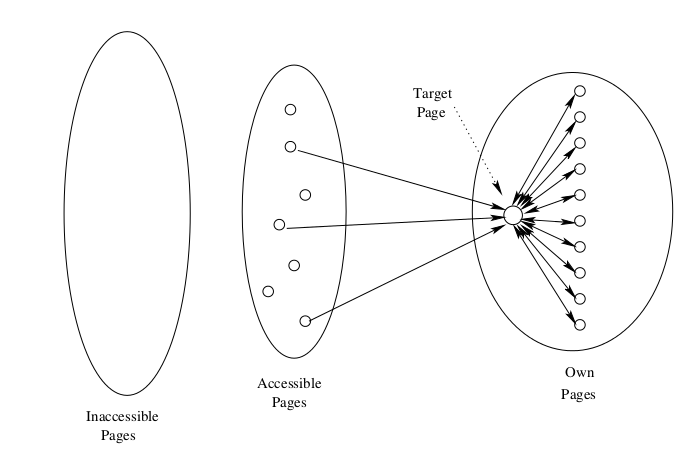
\includegraphics[width=7cm]{SpamFarm.png}
\caption{A spammer's view of the web}
\end{figure}
\end{frame}

\begin{frame}{Spam farm analysis}
\begin{block}{PageRank of the target page}
\begin{itemize}
\item Let $x$ be the input PageRank from the rest of the web, $m$ the number of supporting pages and $n$ the size of the web
\item The PageRank $y$ of $t$ is given by
$ y = \frac{x}{1-\beta^2}+ \frac{\beta}{1+\beta} \frac{m}{n}$
\item If $\beta=.85$ (classical), $\frac{1}{1-\beta^2} = 3.6$ and $\frac{\beta}{1+\beta} = 0.46$
\end{itemize}
\end{block}
\end{frame}

\begin{frame}{TrustRank and Spam Mass}
\begin{block}{TrustRank}
\begin{itemize}
\item Topic sensitive applied to a set of pages deemed trustworthy(inaccessible for the spammers)
\item Trust set determined by humans, or trusted domain names (.gov, .mil in the U.S.)
\end{itemize}
\end{block}
\begin{block}{Spam Mass}
\begin{itemize}
\item Intuition : Portion of the PageRank due to spam
\item Page $p$ with PageRank $r$ and TrustRank $t$
\item Spam Mass of $p = \frac{r-t}{t}$
\item Remove pages with a high Spam Mass from results ordering
\end{itemize}
\end{block}
\end{frame}

\section{Implementation}
\begin{frame}{Efficient representation of Transition Matrices}
  % Quentin
  \begin{block}{URLs and hyperlinks storage}
  \begin{itemize}
    \item Each URLs is associated with an integer
    \item M is sparse, represent it by its non-zero elements
    \item For each column : one integer for the out-degree, one integer per non-zero entry
  \end{itemize}
  \end{block}
\end{frame}

\begin{frame}{Use of MapReduce}
  \begin{block}{First approach}
    \begin{itemize}
      \item Separate v and separate M in k stripes
      \item Use of k map tasks whose sum is the result of a pagerank iteration
      \item The result v' will not fit in main memory either
    \end{itemize}
  \end{block}
  \begin{block}{Second approach : separate M in blocks}
    \begin{itemize}
      \item Separate v in k parts and M in $k^2$ squares.
      \item Use of $k^2$ map tasks, v is transmitted over the network k times
      \item Representing a column of blocks takes more space than a stripe but not too much (max 2 times more because of the repetition of the out degree)
    \end{itemize}
  \end{block}
\end{frame}
\begin{frame}{Application to search engine}
  \begin{itemize}
    \item \textbf{Collect the data} Web crawlers
    \item \textbf{Selection of pages} A page needs to satisfy certain criteria to be considered in the pagerank, then other properties are used to determine (ex : search terms in prominent places)
    \item \textbf{Computation of pagerank} The algorithm described is used to associate a number to each page
    \item \textbf{Determination of the order on the result page} Each search engine has a secret formula in which pagerank plays an important role
    \end{itemize}
\end{frame}

\begin{frame}{Hubs and Authorities}
  \begin{itemize}
    \item Hubs have links to interesting authorities.
    \item Autorities are linked to by good hubs.
  \end{itemize}
  We take $L^T$ which is \emph{exactly} the adjacency matrix.
  \begin{align*}
    a_{k+1} & = \alpha_k L^T h_k\\
    h_{k+1} & = \beta_k  L a_{k+1}
  \end{align*}
  where $\alpha_k, \beta_k$ are scaling factors (since the matrix is no more stochastic)
  such that
  \begin{itemize}
    \item largest element is 1 or
    \item sum of elements is 1
  \end{itemize}
\end{frame}

\begin{frame}
  \begin{thebibliography}{10}
      \beamertemplatebookbibitems
    \bibitem{leskovec2014mining}
      Leskovec, Jure and Rajaraman, Anand and Ullman, Jeffrey David.
      \newblock {\em Mining of massive datasets}.
      \newblock 2014.
      \newblock Cambridge University Press.
      \beamertemplatearticlebibitems
    \bibitem{kitchens1998symbolic}
        Kitchens, Bruce.
        \newblock {\em Symbolic dynamics: one-sided, two-sided and countable state Markov shifts}.
        \newblock 1998.
        \newblock Springer.        
        \bibitem{GooglePaper}
        Stanford University
        \newblock {\em The PageRank Citation Ranking: Bringing Order to the Web}
        \newblock 1998
        \newblock  \url{http://ilpubs.stanford.edu:8090/422/1/1999-66.pdf}
      \beamertemplatearticlebibitems
    \bibitem{ilprints422}
        Lawrence Page and Sergey Brin and Rajeev Motwani and Terry Winograd.
        \newblock {\em The PageRank Citation Ranking: Bringing Order to the Web}.
        \newblock {1999}.
        \newblock {Stanford InfoLab}.
  \end{thebibliography}
\end{frame}


\end{document}

% Sources images :
% Gooooooogle : http://triooti.com/2014/08/23/google-nous-cache-des-informations-dans-les-recherches/
% Web graph : matthewgress.com
% Pagerank : wikipedia
